%%%%%%%%%%%%%%%%%%%%%%%%%%%%%%%%%%%%%%%%%%%%%%%%%%%%%
%%% Task 3 %%%%%%%%%%%%%%%%%%%%%%%%%%%%%%%%%%%%%%%%%%
%%%%%%%%%%%%%%%%%%%%%%%%%%%%%%%%%%%%%%%%%%%%%%%%%%%%%
\task{Transformer model parameterization}

%%%%%%%%%%%%%%%%%%%%%%%%%%%%%%%%%%%%%%%%%%%%%%
\taskGerman{Transformator Modellparametrierung}
%%%%%%%%%%%%%%%%%%%%%%%%%%%%%%%%%%%%%%%%%%%%%%
The transformer designed in task 1 has been manufactured, and experimental tests must be carried out to determine its T-type equivalent circuit model parameters.

\begin{hintblock}
	if you are not able to solve task 1, use $ü = 35$ as substitute results for the subsequent tasks.
\end{hintblock}

\begin{germanblock}
	Der in Aufgabe 1 entworfene Transformator wurde nun hergestellt, und es müssen experimentelle Tests durchgeführt werden, um seine T-Typ-Ersatzschaltbildparameter zu ermitteln.
\end{germanblock}

\begin{germanhintblock}
	Falls Sie kein Ergebnis für Aufgabe 1 ermitteln können, verwenden Sie $ü = 35$ für die nachfolgenden Aufgaben.
\end{germanhintblock}

\subtask{Draw the equivalent circuit diagram for the open-circuit test (incl. labeling of components, voltages and currents).}{1}

\subtaskGerman{Zeichnen Sie das Ersatzschaltbild für den Leerlaufversuch (inklusive Beschriftung der Komponenten, Spannungen und Ströme).}

\begin{solutionblock}
	The ECD is shown in \autoref{fig:sol_open_circuit_test}.
	\begin{solutionfigure}[h!]
		\centering
		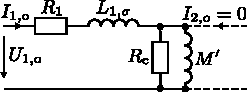
\includegraphics[width=0.45\textwidth]{fig/sol_Transformer_open_circuit_test.pdf}
		\caption{ECD for the open-circuit test.}
		\label{fig:sol_open_circuit_test}
	\end{solutionfigure}

\end{solutionblock}


\subtask{In the open-circuit test, $U_{1,\mathrm{o}}=\SI{230}{\volt}$, $P_{1,\mathrm{o}}=\SI{10}{\watt}$, and $S_{1,\mathrm{o}}=\SI{15}{\volt\ampere}$ were measured. Determine the iron loss resistance $R_\mathrm{c}$ and the mutual inductances $M'$ and $M$ (referred to the primary side and unreferred). Neglect ohmic losses and stray inductances.}{3}

\subtaskGerman{Bei dem Leerlaufversuch wurden eingansseitig eine Wirkleistung von $P_{1,\mathrm{o}}=\SI{10}{\watt}$ sowie Scheinleistung von $S_{1,\mathrm{o}}=\SI{15}{\volt\ampere}$ gemessen. Unter Vernachlässigung der ohmschen Verluste sowie der Einflüsse der Streuinduktivitäten sind der Eisenverlustwiderstand $R_\mathrm{c}$ sowie die Gegeninduktivität $M'$ und $M$ (transformiert auf die Primärseite sowie untransformiert) zu bestimmen.}

\begin{solutionblock}
	Based on the made assumptions, the measured active input power is dissipated as iron losses yielding
	$$
		R_\mathrm{c} = \frac{U^2_{1,\mathrm{o}}}{P_{1,\mathrm{o}}} = \SI{5290}{\ohm}.
	$$
	Based on the measured input powers, the power factor for the open-circuit test is
	$$
		\cos(\varphi_\mathrm{o}) = \frac{P_{1,\mathrm{o}}}{S_{1,\mathrm{o}}} = 0.67 \quad \Leftrightarrow \quad \varphi_\mathrm{o} = \SI{84}{\degree}.
	$$
	The input current during the open-circuit test must have been
	$$
		I_{1,\mathrm{o}} = \frac{S_{1,\mathrm{o}}}{U_{1,\mathrm{o}}} = \SI{0.065}{\ampere}.
	$$
	The reactance of the open-circuit transformer is
	$$
		X_\mathrm{o} = \frac{U_{1,\mathrm{o}}}{I_{1,\mathrm{o}}}\frac{1}{\sin(\varphi_\mathrm{o})} = Z_\mathrm{0} \frac{1}{\sin(\varphi_\mathrm{o})} = \SI{4731.5}{\ohm}.
	$$
	This reactance must be identical to the reactance provided by the transformed mutual inductance as the stray inductance impact is neglected:
	$$
		\omega M' = X_\mathrm{o} \quad \Leftrightarrow \quad M' =\frac{X_\mathrm{o}}{\omega} = \SI{15.06}{\henry}.
	$$
	Based on the estimated transformation ratio, the original mutual inductance yields
	$$
		M = \frac{1}{\ddot{u}}M' = \SI{0.37}{\henry}.
	$$
\end{solutionblock}




\subtask{During a follow-up short-circuit test with $U_{\mathrm{1,s}}=\SI{3.4}{\volt}$, $I_{\mathrm{1,s}}=\SI{0.5}{\ampere}$ and $P_{\mathrm{1,s}}=\SI{1.6}{\watt}$ were measured. Determine $R_1 = R'_2$ and the untransformed $R_2$, as well as $L_{1,\sigma}=L'_{2,\sigma}$ and the untransformed $L_{2,\sigma}$. Neglect the mutual inductance.}{3}

\subtaskGerman{Bei einer anschließenden Kurzschlussprüfung mit $U_{\mathrm{1,s}}=\SI{3,4}{\volt}$ wurden folgende Messwerte ermittelt: $I_{\mathrm{1,s}}=\SI{0,5}{\ampere}$, $P_{\mathrm{1,s}}=\SI{1,6}{\watt}$. Bestimmen Sie $R_1 = R'_2$ sowie das untransformierte $R_2$. Bestimmen Sie ebenfalls $L_{1,\sigma}=L'_{2,\sigma}$ sowie das untransformierte $L_{2,\sigma}$. Vernachlässigen Sie hierbei den Einfluss der Gegeninduktivität.}

\begin{solutionblock}
	The short-circuit impedance is
	$$
		Z_\mathrm{s} = \frac{U_{\mathrm{1,s}}}{I_{\mathrm{1,s}}} = \SI{6.8}{\ohm},
	$$
	while the corresponding power factor is
	$$
		\cos(\varphi_\mathrm{s}) = \frac{P_{\mathrm{1,s}}}{U_{\mathrm{1,s}}I_{\mathrm{1,s}}} = 0.94 \quad \Leftrightarrow \quad \varphi_\mathrm{s} = \SI{19.9}{\degree}.
	$$
	Separating the real and imaginary part of the impedance, one receives
	$$
		R_1 + R'_2 = Z_\mathrm{s}\cos(\varphi_\mathrm{s}) = \SI{6.4}{\ohm} \quad \Longrightarrow \quad R_1 = R'_2 =  \SI{3.2}{\ohm}
	$$
	and
	$$
		(L_{1,\sigma} + L'_{2,\sigma})\omega = Z_\mathrm{s}\sin(\varphi_\mathrm{s}) = \SI{721.9}{\ohm} \quad \Longrightarrow \quad L_{1,\sigma} = L'_{2,\sigma} =  \SI{3.6}{\milli\henry}.
	$$
	The untransformed secondary values result in
	$$
		R_2 = \frac{1}{\ddot{u}^2} R'_2 = \SI{2}{\milli\ohm}, \quad L_{2,\sigma} = \frac{1}{\ddot{u}^2} L'_{2,\sigma} = \SI{2.2}{\micro\henry}.
	$$
\end{solutionblock}
